\documentclass[a4paper]{article}
\usepackage{url}
\usepackage[utf8]{inputenc}
\usepackage{fancyvrb}
\usepackage{hyperref}
\addtolength{\textheight}{1cm}

\title{Posłowie na Sejm RP 7 kadencji wg stażu}
\author{Tomasz Przechlewski}
\usepackage{Sweave}
\begin{document}
\maketitle

\section{Dane}
Plik \url{sejm7_wg_stazu_wieku.csv} zawiera m.in. informacja o~liczbie kadencji (staż)
na jaką został wybrany poseł (kolumna \texttt{kadencje}). 
Wartość minimalna w~tej kolumnie wynosi $1$ dla posła wybranego po raz pierwszy do Sejmu~7 kadencji.

\begin{Schunk}
\begin{Sinput}
> library(ggplot2);
> ## Pierszy wiersz pliku CSV: imnz;rokur;klub;kadencje
> poslowie <- read.csv("sejm7_wg_stazu_wieku.csv", sep = ';',  header=T);
\end{Sinput}
\end{Schunk}

%Dane zostały pobrane ze strony \url{http://www.sejm.gov.pl/Sejm7.nsf/poslowie.xsp}.

\section{Staż posłów wybranych do Sejmu}

Posłowie~7 kadencji wg.~średniego stażu (w~podziale wg przynależności klubowej):

\begin{Schunk}
\begin{Sinput}
> tapply (poslowie$kadencje, poslowie$klub, mean);
\end{Sinput}
\begin{Soutput}
   niez.      PiS       PO      PSL       RP      SLD 
2.500000 2.737179 2.497585 3.642857 1.097561 3.615385 
\end{Soutput}
\begin{Sinput}
> # http://ww2.coastal.edu/kingw/statistics/R-tutorials/descriptive.html
> table(poslowie$klub, poslowie$kadencje)
\end{Sinput}
\begin{Soutput}
         1  2  3  4  5  6  7
  niez.  1  0  0  1  0  0  0
  PiS   48 26  5 74  2  1  0
  PO    50 82  1 72  1  0  1
  PSL    5  5  4  5  2  4  3
  RP    39  1  0  1  0  0  0
  SLD    5  3  0 11  5  0  2
\end{Soutput}
\end{Schunk}

Średni staż posłów w~poszczególnych klubach przedstawia rysunek~\ref{srstaz}

\begin{figure}[!tbh]
\begin{Schunk}
\begin{Sinput}
> p0 <- ggplot(data=poslowie,aes(klub,kadencje))+geom_boxplot()
> print(p0);
\end{Sinput}
\end{Schunk}
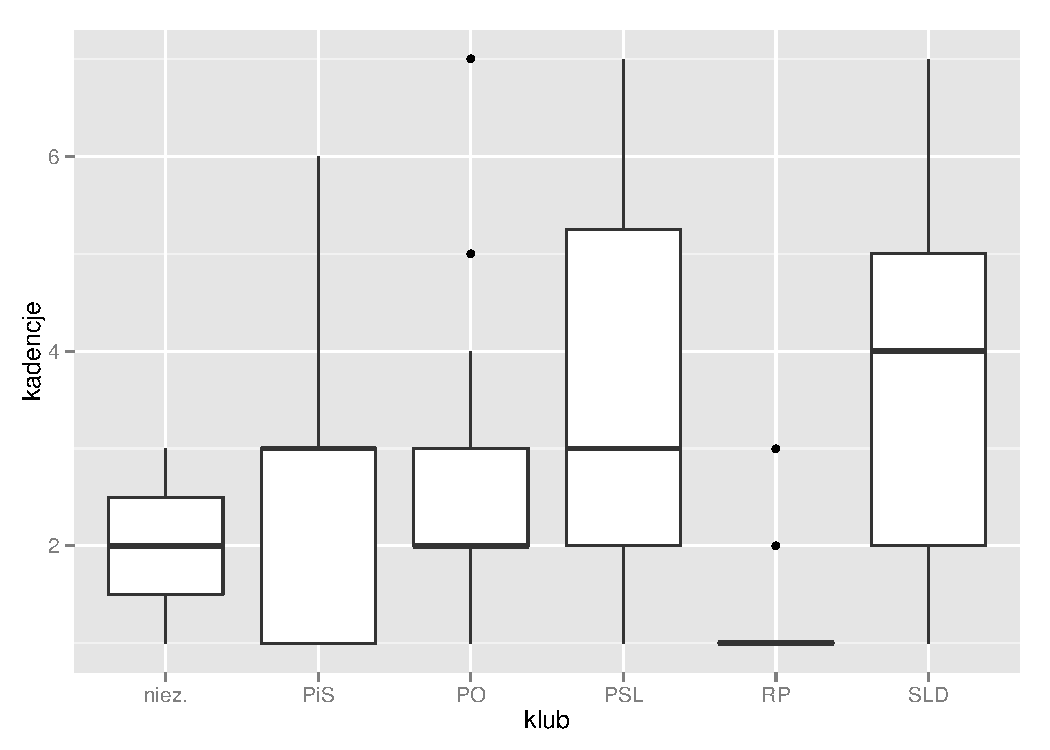
\includegraphics{sejm7_wg_stazu_wieku-srstaz}
\caption{Średni staż posłów (wykres pudełkowy) \label{srstaz}}
\end{figure}


%%
\section{Wiek a liczba kadencji posłów do Sejmu}

Wiek posłów jest liczony jako różnica między rokiem 2011, w~którym odbyły się wybory, a~rokiem urodzenia.
Na rysunku~\ref{wiekstazalt} przedstawiono zależność pomiędzy liczbą kadencji (łącznie z~tą, na którą poseł
został wybrany) a~wiekiem posła.

\begin{figure}[!tbh]
\begin{Schunk}
\begin{Sinput}
> p1 <- qplot(kadencje, wiek, data=poslowie, facets= klub ~ ., 
+              position = position_jitter(w = 0.2, h = 0.2) );
> print(p1);
\end{Sinput}
\end{Schunk}
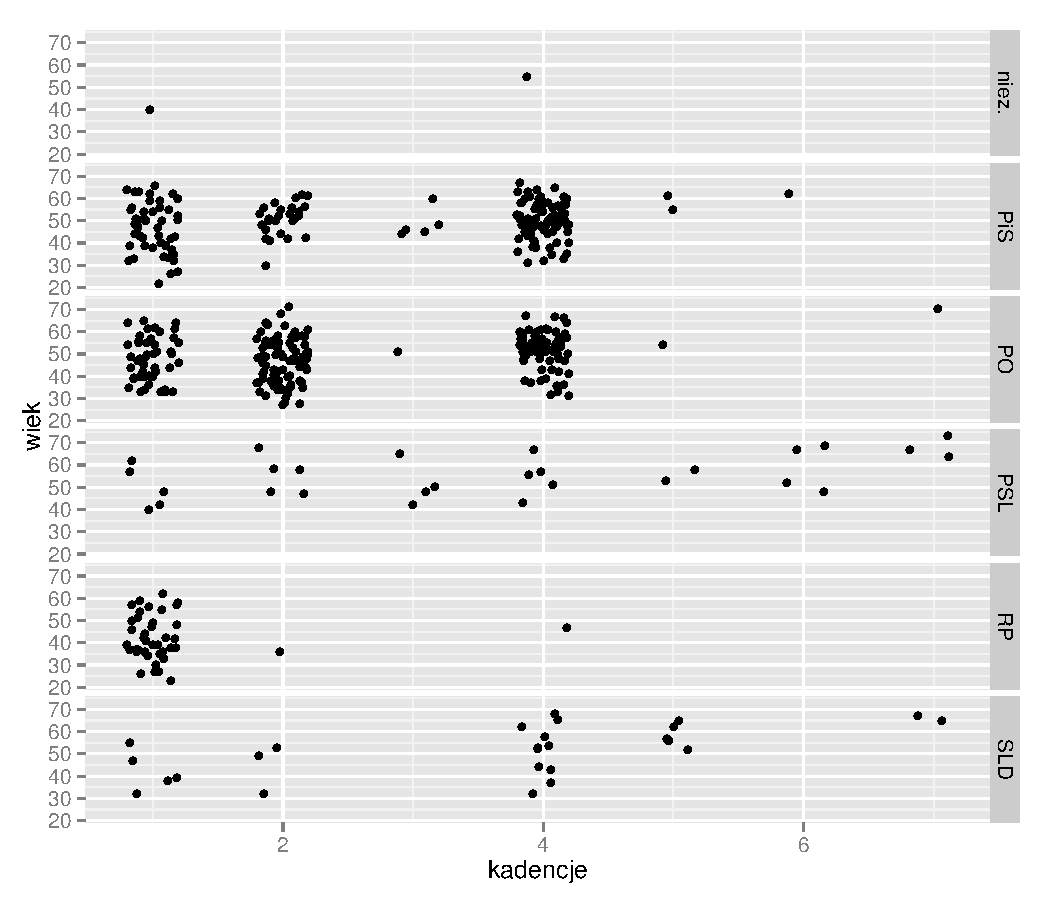
\includegraphics{sejm7_wg_stazu_wieku-wiekstazalt}
\caption{Zależność między wiekiem a liczbą kadencji\label{wiekstazalt}}
\end{figure}

Rysunek~\ref{wiekstazaltalt} przedstawia to samo co~rysunek~\ref{wiekstazalt} tylko wyłączono
parametr \texttt{jitter}. Pozostawiamy czytelnikowi decyzję, która wersja jest bardziej zrozumiała.

\begin{figure}[!tbh]
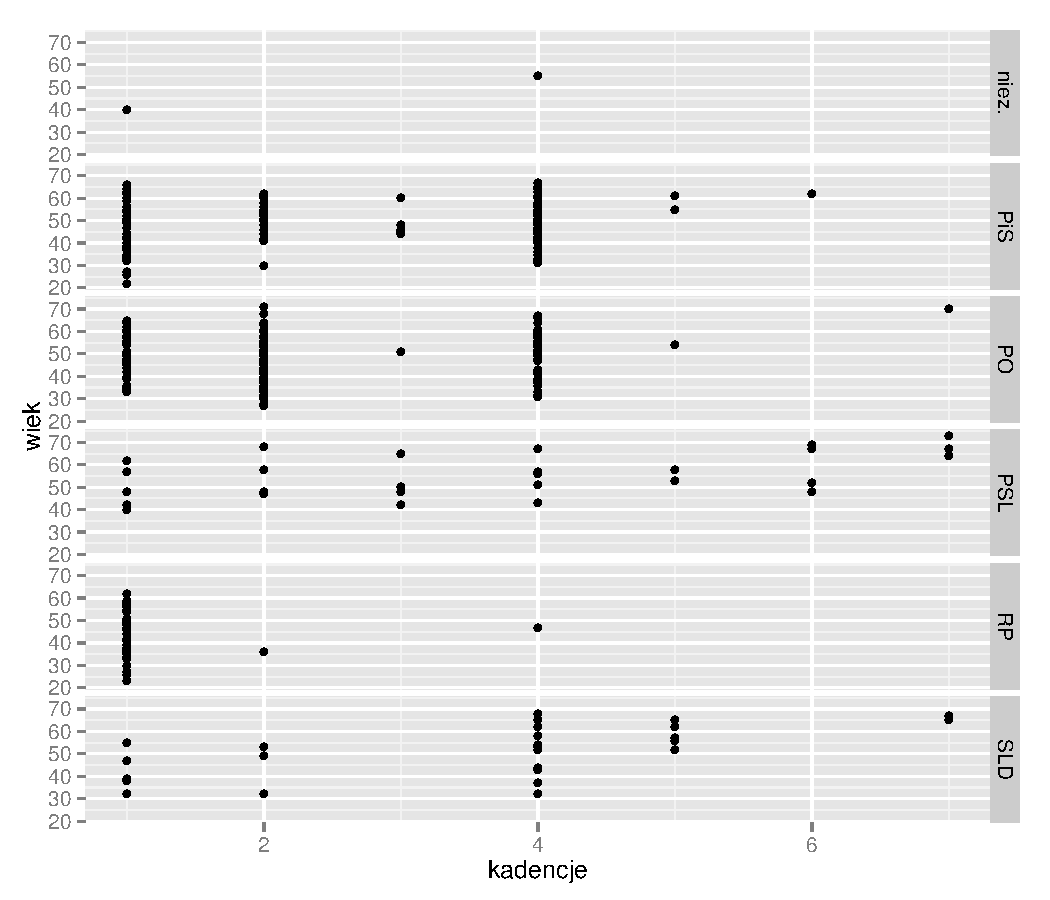
\includegraphics{sejm7_wg_stazu_wieku-wiekstazaltalt}
\caption{Zależność między wiekiem a liczbą kadencji \label{wiekstazaltalt}}
\end{figure}

Rysunek~\ref{wiekstaz} zawiera 
wszystkie dane z~rysunków~\ref{wiekstazalt} na jednym wykresie. Poszczególne
kluby są oznaczone kolorami i~różnymi symbolami. Rysunek jest nieczytelny -- zawiera zbyt dużo danych.

\begin{figure}[!tbh]
\begin{Schunk}
\begin{Sinput}
> p3 <- qplot(wiek, kadencje, data=poslowie, shape=klub, color=klub, 
+             position = position_jitter(w = 0.2, h = 0.2));
> print(p3);
\end{Sinput}
\end{Schunk}
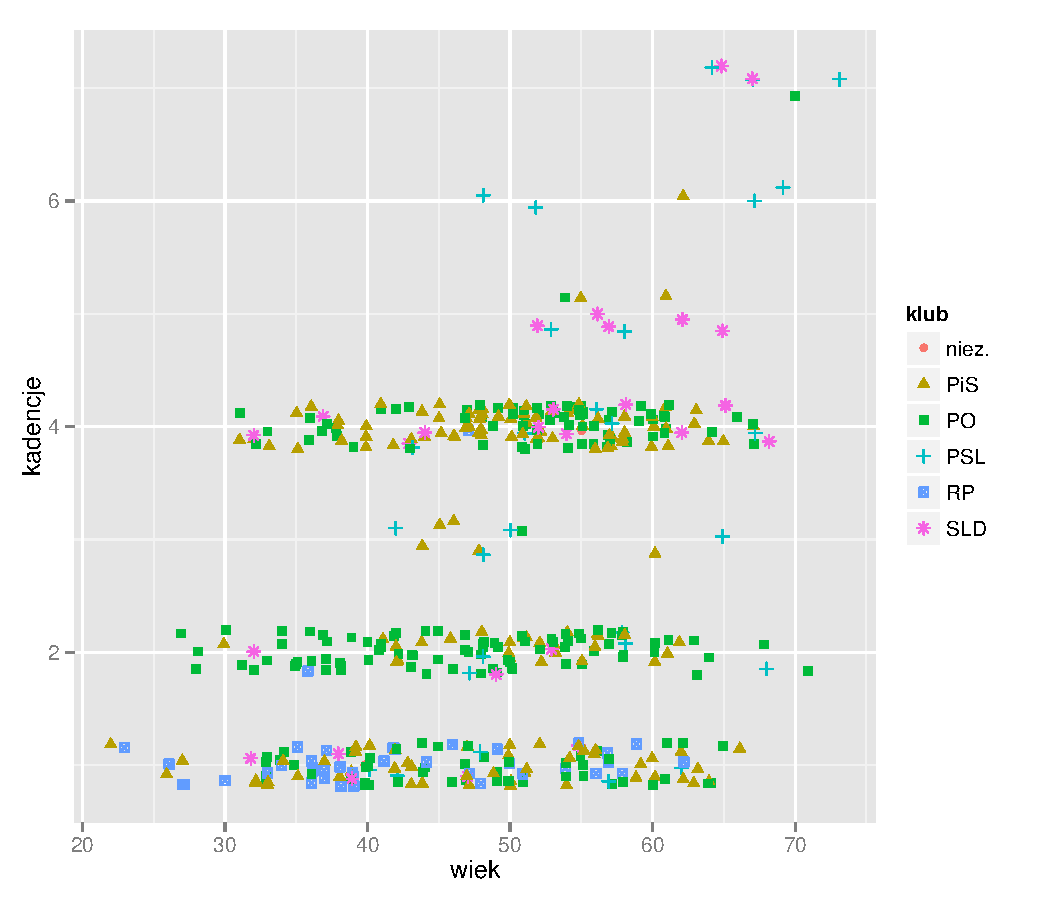
\includegraphics{sejm7_wg_stazu_wieku-wiekstaz}
\caption{Zależność między wiekiem a liczbą kadencji\label{wiekstaz}}
\end{figure}

\end{document}
